\documentclass[]{article}
\usepackage{graphicx}
\usepackage{pdfpages}
\usepackage[margin=1in]{geometry}
\raggedright
\begin{document}

\title{ds2 hw2}
\author{Nick Strayer}
\date{\today}
\maketitle

Code for each problem is given in \texttt{problem\_number.py}

\begin{enumerate}
\item This was relatively straightforward. A couple of the problems that I ran into along the way: 

{\large What tool to use:}
\begin{itemize}
\item I originally tried using \textbf{requests} but the format didn’t work with Tycho (at least in the time I spent with it.) It seemed like Tycho was particular about the order of the parameters in the query and requests couldn’t care less. 

\item I eventually went with good-ol-fashioned \textbf{urllib.} I did this because it was the method that was used in the example on the Tycho website. I lost the ability to fail gracefully but Tycho actually nicely fails in the output anyways so it was fine. 
\end{itemize}

{\large How to feed in the parameters: }

\begin{itemize}
\item It wasn’t super clear if Tycho wanted individual states for the state query, and if it did, if it wanted them given in “loc” or “state” (seems more obvious now looking back on it.) Through trial and error this was figured out. 
\end{itemize}

{\large How to store the data:}

\begin{itemize}
\item Did I want to aggregate the data into individual csv’s for each state or disease or what? Eventually, I decided to simply get everything in as fine a resolution as possible because space is cheap and later processing would be easier if I choose to switch my methods. 
\end{itemize}

{\large Messed up disease names:}
\begin{itemize}
\item The first time that I ran the script I incorrectly queried for Chickenpox and Whooping cough. I didn’t realize that you needed to name them explicitly (i.e. with their formal name in square brackets).
\item I changed their names and re-ran the script only looping over the messed up diseases. \textbf{Lines 43 to 48 in problem1.py}.
\end{itemize}

\vspace{2em}
\item The age old question of how to represent data! I am choosing to go summed by the whole country as state boundaries, in my opinion, especially for something like this are rather arbitrary. No-one*  looks back and remembers how badly a disease hit Ohio in the 1920’s, (an exception would be for something like AIDS in San Fransisco in the 1980’s, but we aren’t looking at that data.) 

I read in all of the files grabbed in problem 1, then concatenated them by disease, grouped by year, then summed to get the whole country average. \textbf{20 to 27 in problem2.py}
\newpage
{\large Output:}

\centerline{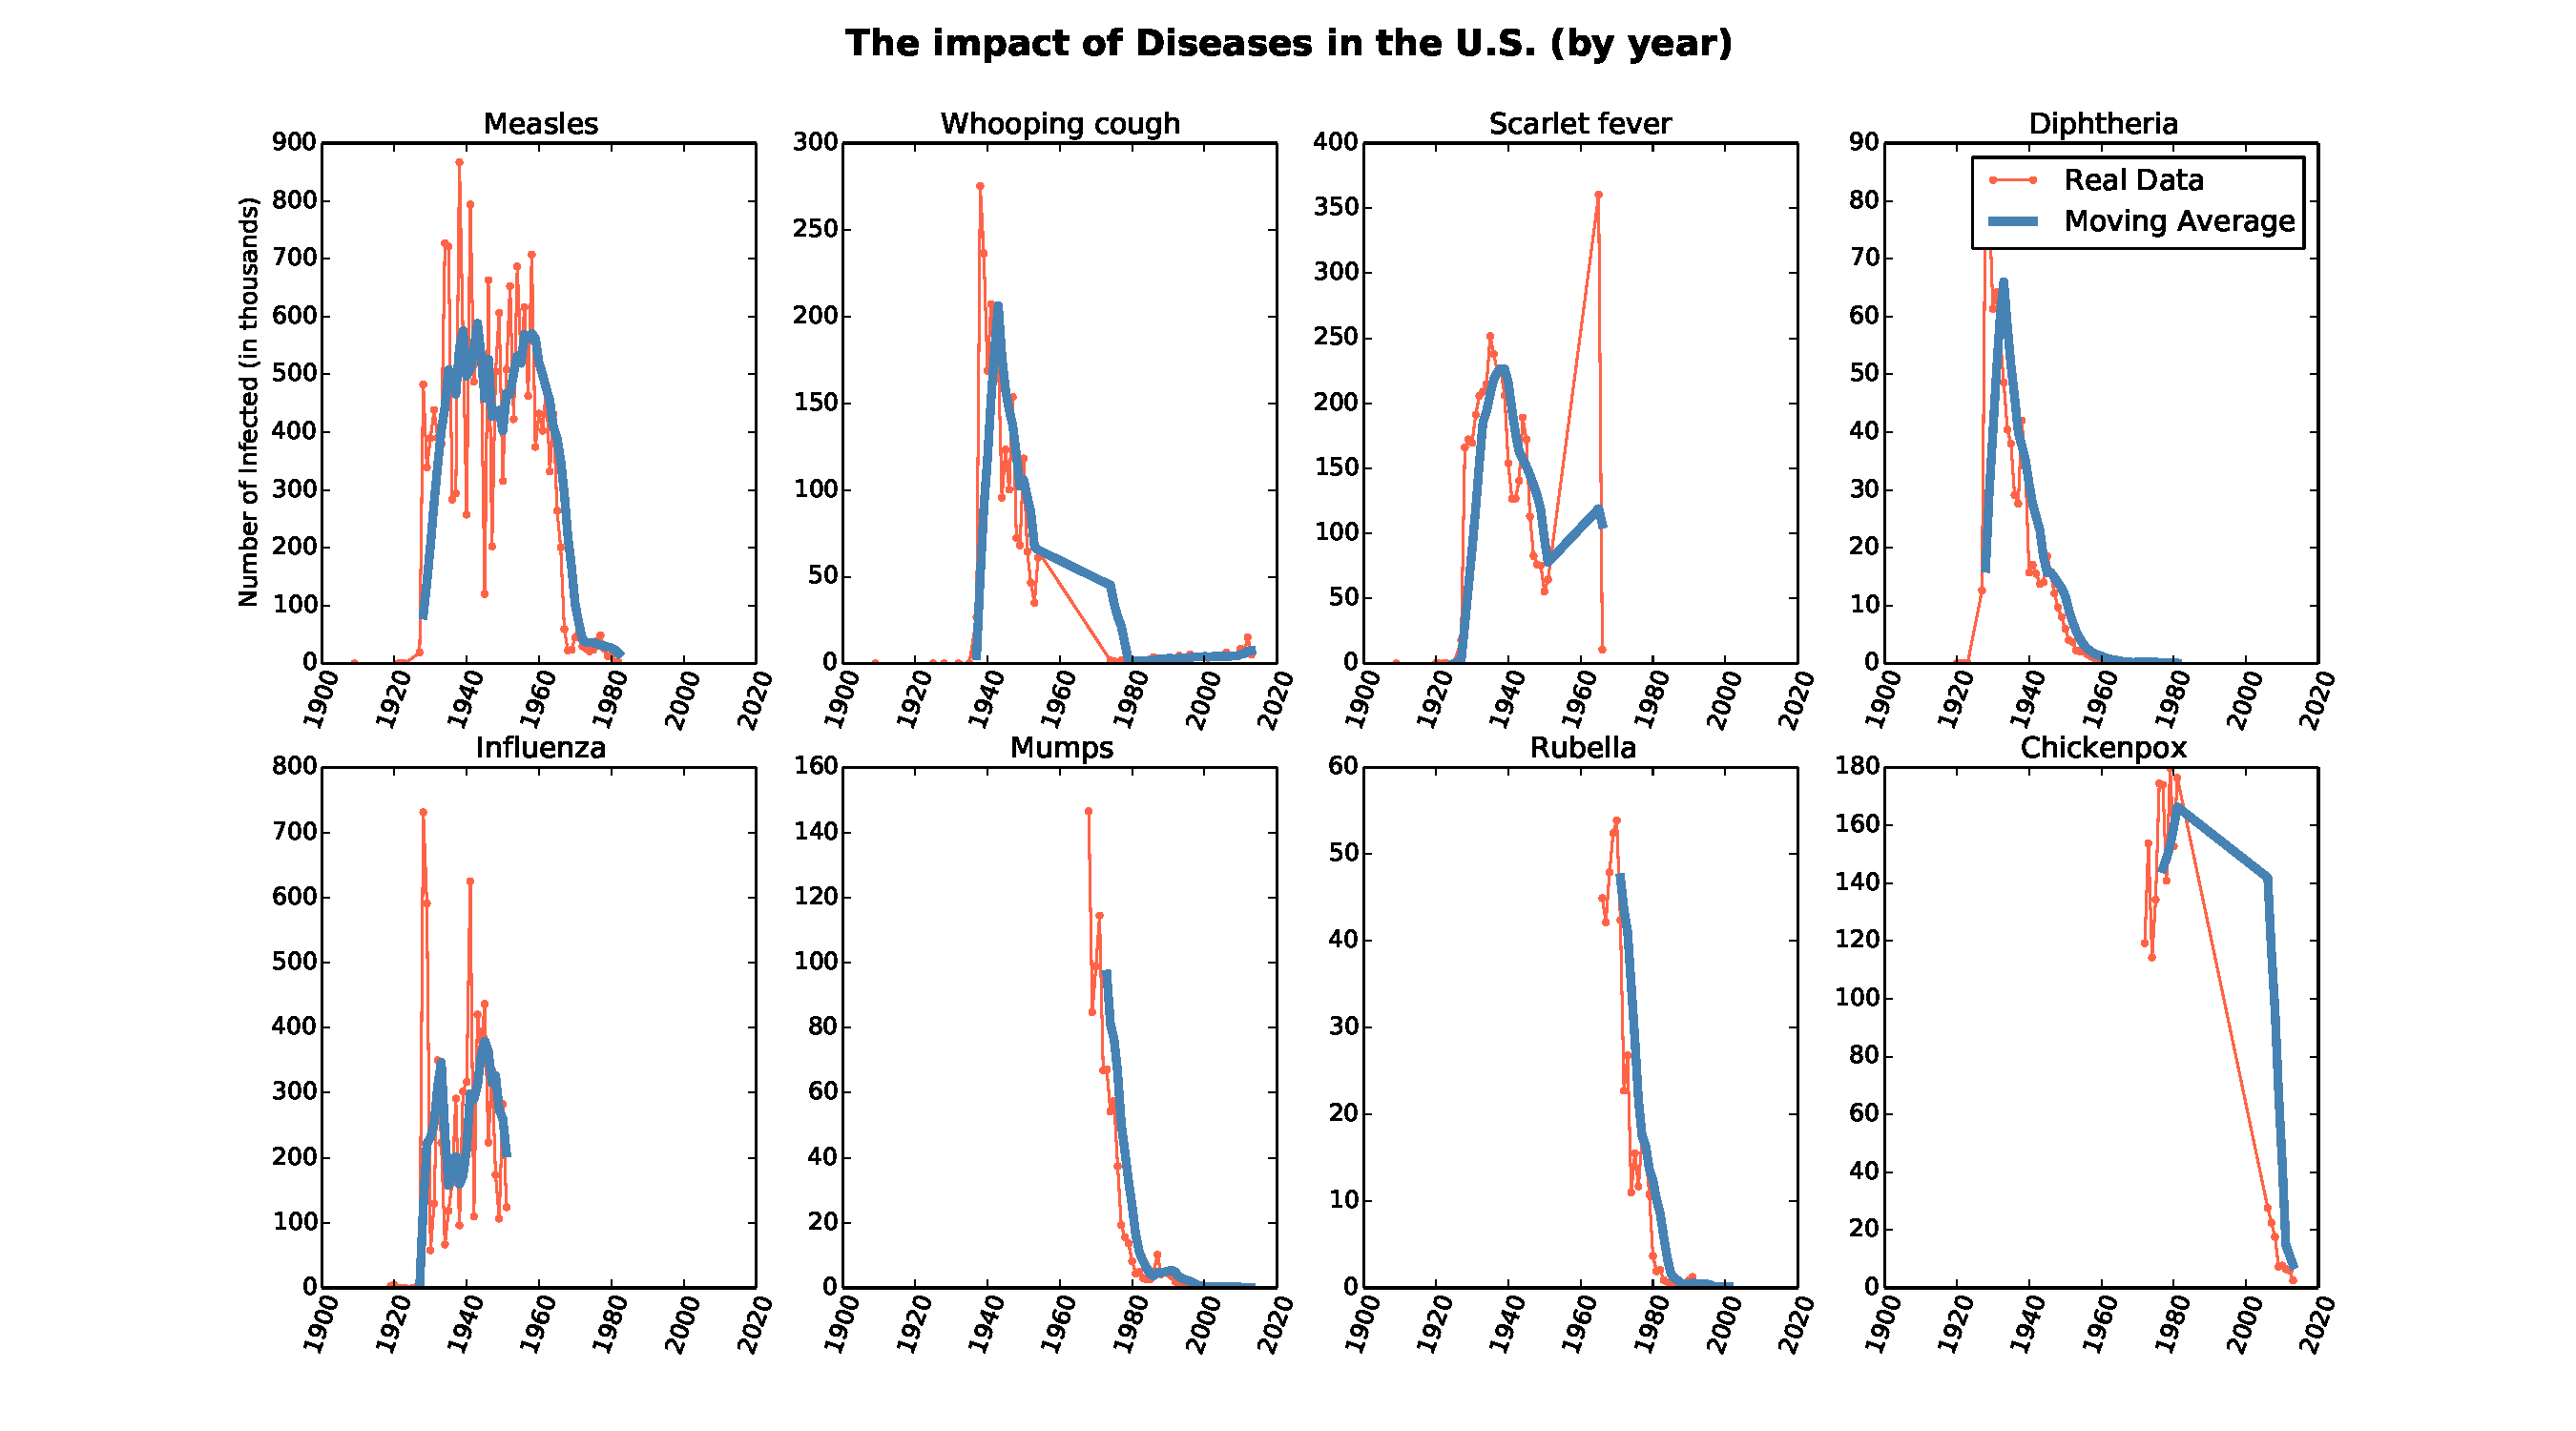
\includegraphics[scale = 0.4]{figures/diseaseCasesByYear.pdf}}


\textbf{Note:} This also made me aware of the problems with the death data. I am not sure why, but there seems to be a big gulf between the amount of info project Tycho has on cases vs. deaths. For this reason only cases were plotted. The few queries that did return death data contained too sparse a data to provide any meaningful plot or takeaway. 

\vspace{2em}
\item A quick google search shows that this question could literally fill multiple theses, so, I will heed the advice given and make something as simple as possible. 

I chose to find the difference in values between every successive measurement. I.e. \texttt{|value\_i - value\_i+1|}. My thought process is that this will help us see the fluctuations. The part of the resulting output (when plotted) that will indicate ability to be predicted, will be the flatness of the line. This will help the comparisons of diseases with different orders of magnitude, since the flatness is relative. 

\begin{verbatim}
def predictabilityIndex(diseaseCounts):
    differenceList = []
    for i in range(len(diseaseCounts) - 1): 
        change = abs(diseaseCounts[i] - diseaseCounts[i+1])
        differenceList.append(change)
        
    return differenceList
\end{verbatim}


After I did this I chose to do linear regression on the output. Unlike normal linear regression though, the goal, at least for predictability, would be to have the slope of the line be zero, so in our case, we want the smallest R-Values as possible. These are the results: 

\centerline{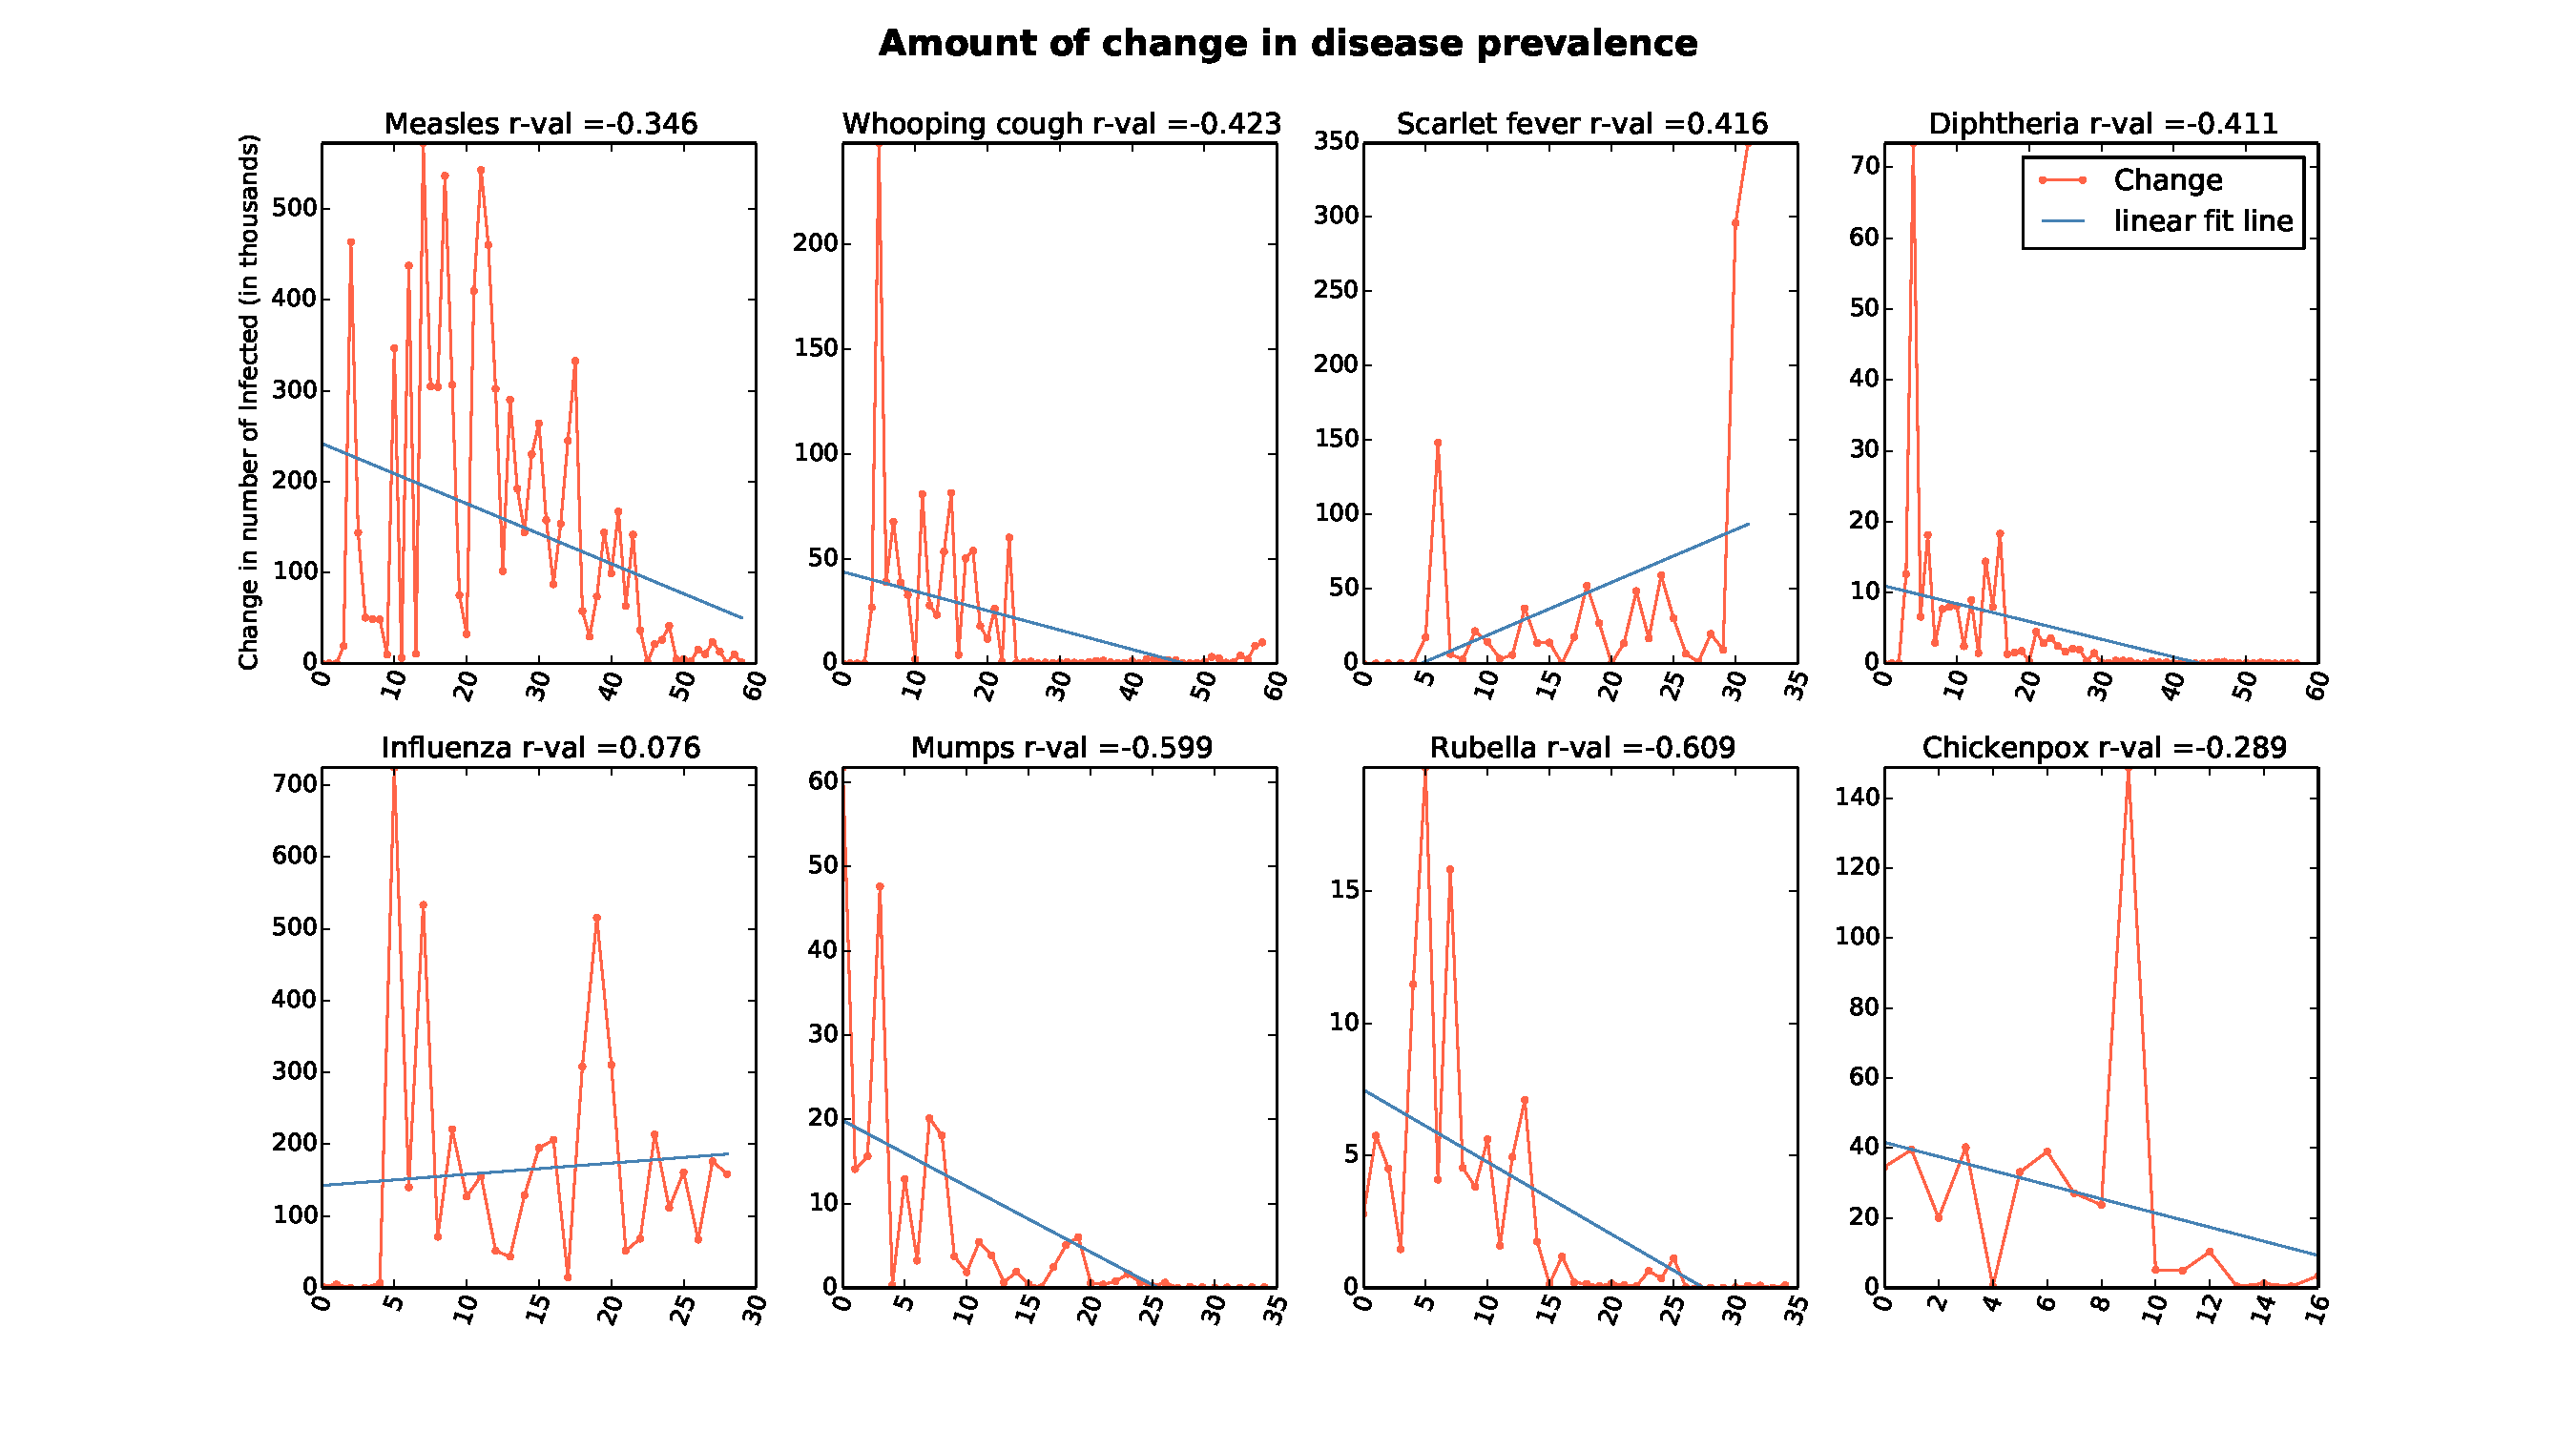
\includegraphics[scale = 0.4]{figures/problem3Output.pdf}}

{\large Applying to polio}

I went back and to the homework 1 work and modified the plotting portion of my iPython notebook to do this same thing with the polio data. (I have ditto-ed the whole hw01 directory into this homework directory and modified it there):

\begin{verbatim}
import scipy.stats as sp
import matplotlib.ticker as ticker
steelBlue = "#4682b4"
niceRed   = "#ff6347"

def predictabilityIndex(diseaseCounts):
    ...

def findLinearFitLine(changeAmount_list):
   ...

changeInPolio = predictabilityIndex(list(polioByYear["U.S"]))
fig = plt.figure(figsize=(12,8))
plt.plot(changeInPolio, niceRed,marker='.')
ax = fig.add_subplot(1,1,1)
rVal, pVal, linearFitLine = findLinearFitLine(changeInPolio)
plt.plot(linearFitLine, steelBlue)
\end{verbatim}
\newpage
Here is the output: 

\centerline{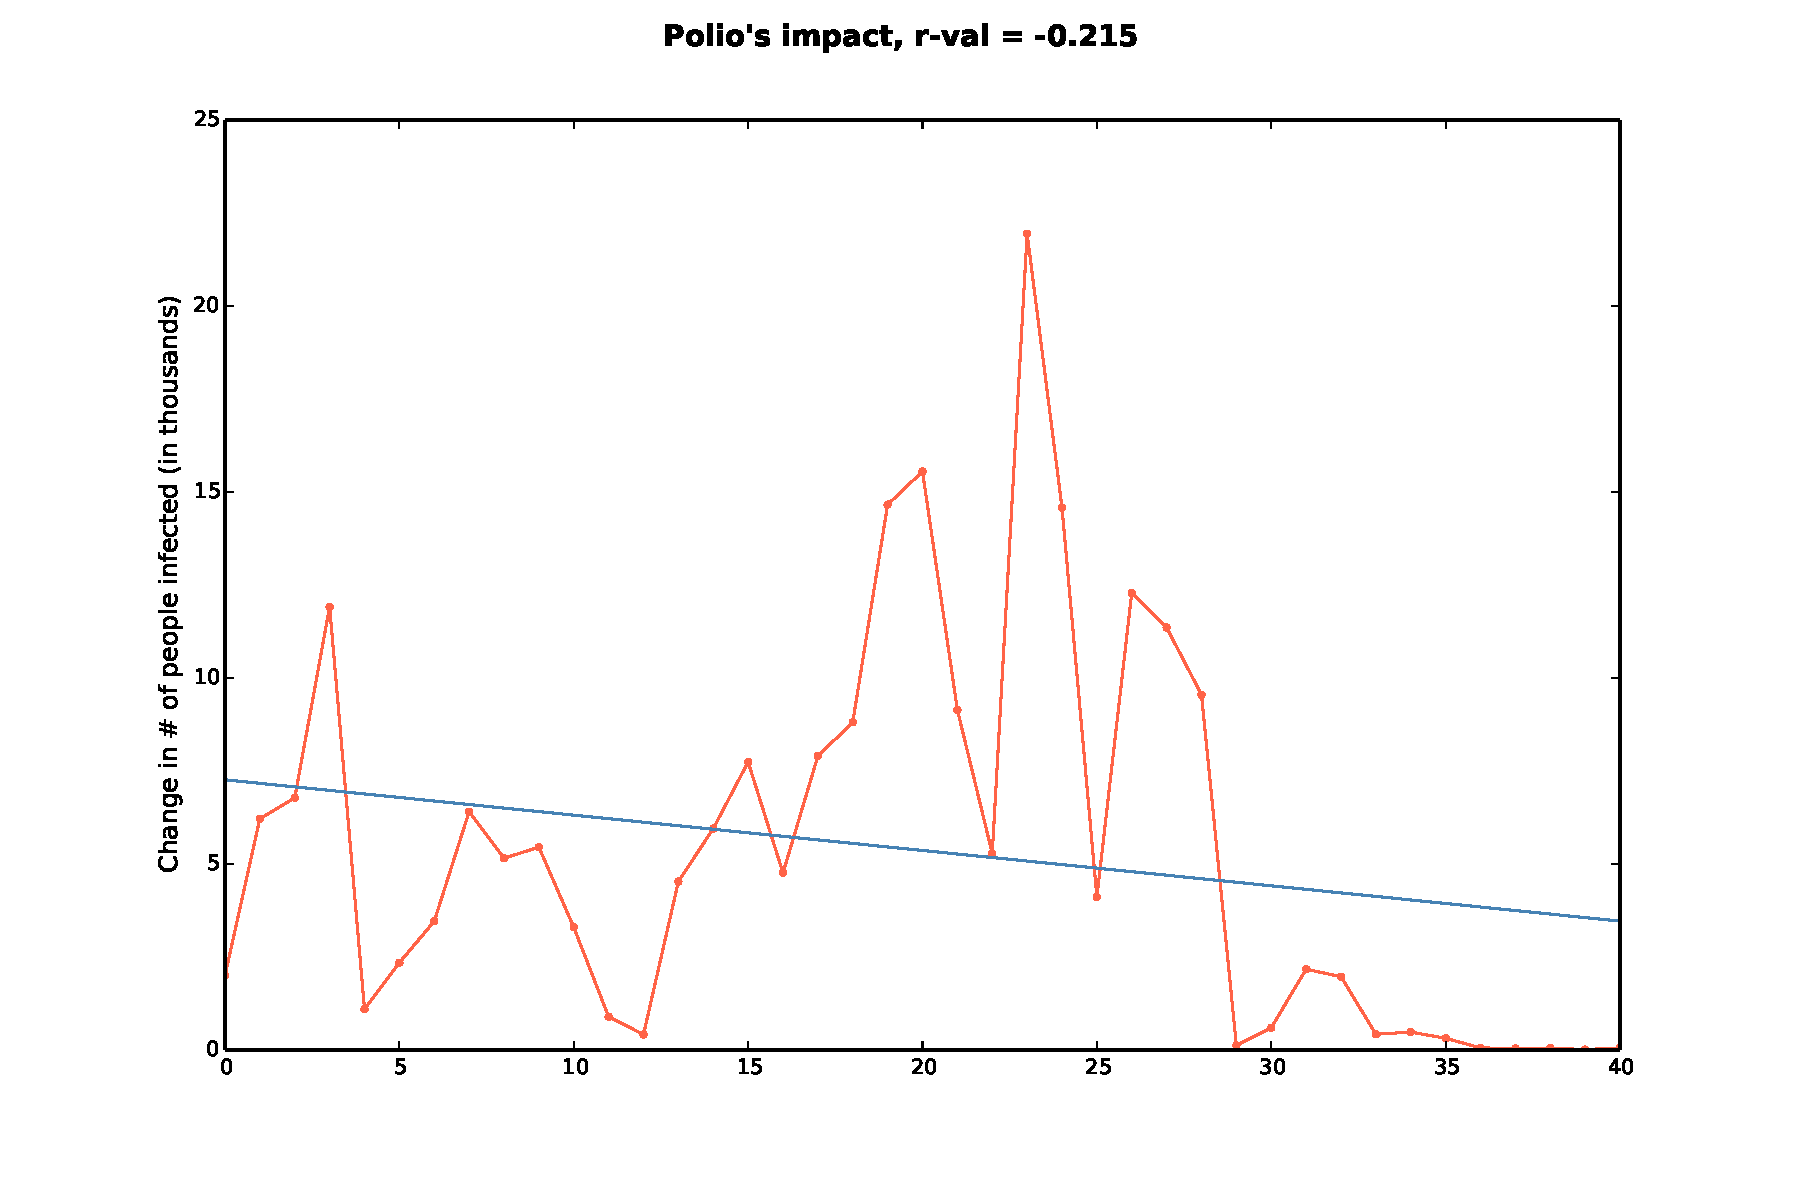
\includegraphics[scale = 0.4]{figures/polioChange.pdf}}

{\large Interpretation:}

From this comparison we can see that polio sits relatively in the bottom of the pack in terms of its r-val. But nothing is substantially different, and influenza for example is way more predictable. 
\end{enumerate}

\vspace{2em}
{\large Bonus question:}

You could estimate incidence rate if you took into account the average duration of the disease and the death rate of the disease. However, given the scope of this homework this is not realistic. 

\vspace{1em}

For one, the death rates would have to be more robust. In their current form there simply isn't enough data to reliably estimate the incidence rates. Also, we don't have information on average disease duration. These data however, could be gotten relatively easy, but I have three more homework assignments that I need to do, so it is effectively impossible. 
\end{document}